\clearpage
\chapter{Physics Object Definitions}\label{sec:objects}
%reconstruction algorithms, isloation, cleaning, IDs, particle flow

In this section, we provide the definitions of physics objects used in the analysis.
The analysis uses 2 main CMS reco objects: muons, jets.
Photons do not show anywhere in our signal process.
$\tau$'s of our signal process can decay into electrons with same probability as into muons. 
However, the analysis uses b-parking and only targets the muon decay mode of the tau.
Electrons are not interest of our analysis either.

Although the signal's final decay involves $\tau$ lepton, we do not use the CMS reconstructed $\tau$.
Given that $\tau$ decay results into many different objects (muon, electron, and different combinations of hadrons) as shown in figure \ref{fig:tdecay}, the CMS uses a special reconstruction algorithm for $\tau$ object.
Particle-Flow jets (PFjets), which are jets with all particle identification information within the jet, are the starting point for the $\tau$ reconstruction.
With $\pi^{0}$ reconstructed in ECAL as a strip, the Hadronic-Plus-Strip (HPS) algorithm reconstructs $\tau$ (at 60\% efficiency in Run 1) when a charged hadron and a strip is reconstructed in the PFJet \cite{HPS}.
Our signal process tau lepton decays into muon, in a leptonic mode, for the trigger.
For other tau leptons in the signal process, we approach purely tracker oriented method with regions of Interest for our analysis.
Direct usage of tau leptons in the analysis is accompanied by division of several different sub-channels ($\mu$,e,had), which result in 27 ($3^{3}$) different combinatorics. 

We use muon leptons, jets, and only tracks (ROIs) for this analysis.
\section{Muons}\label{sec:muons}
The analysis sources the SlimmedMuons collection from the MINIAOD MC datasets to produce {\tt selectedPatMuons}.
Muon objects are required to have 
\begin{itemize}
  \item $pT$ $\geq$ 12 GeV to reach BPH trigger plateau
  \item $|\eta|$ $\leq$ 1.5 for L1 seed $|\eta|$ cut in BPH trigger
  \item reco::Muon object matched to the BPH trigger object
  \item Pass the Loose ID criterion (isLooseMuon) as described in the Muon POG~\cite{muonpog}.
\end{itemize}

\begin{figure}[h!]
  \caption{Data/MC of muon objects pT and $\eta$}
  \label{fig:muons}
  \centering
  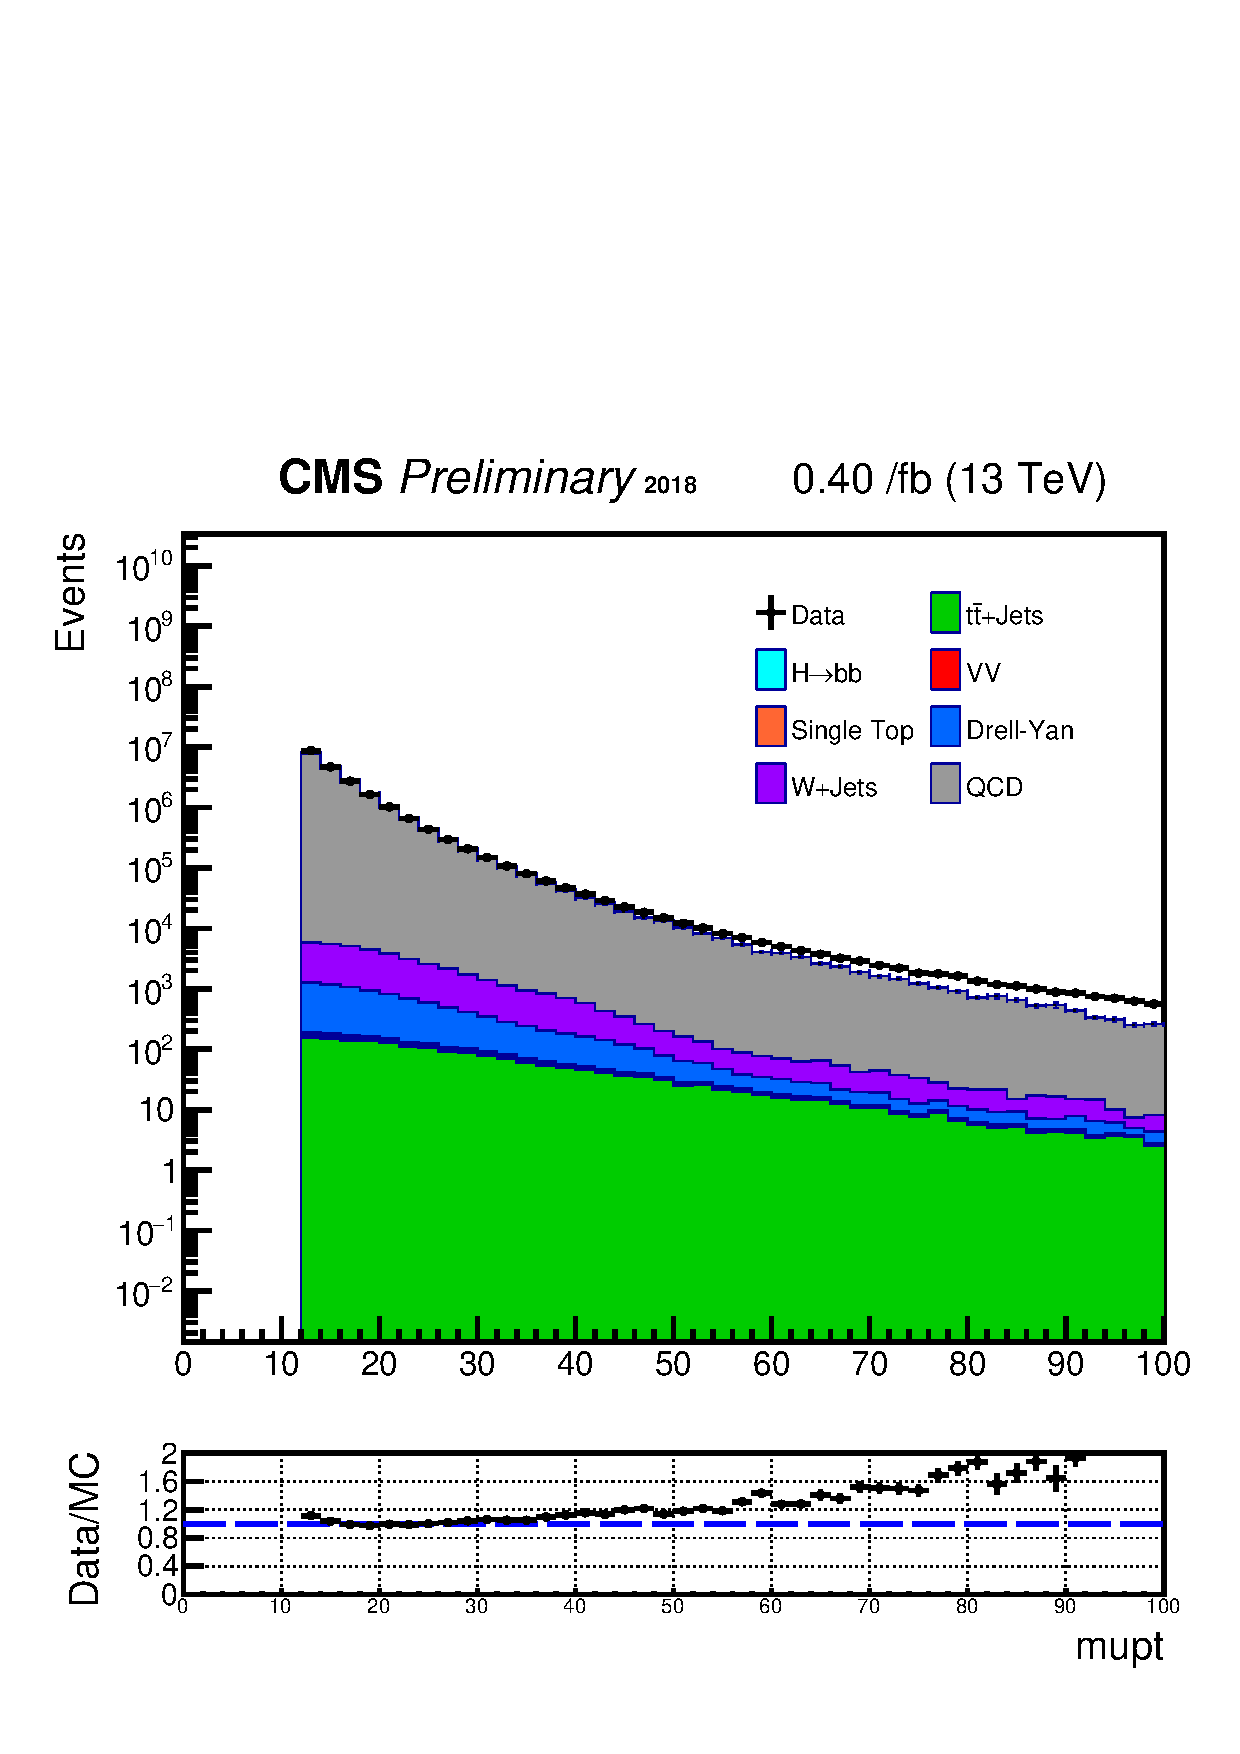
\includegraphics[width=0.47\linewidth]{figs/Data_AnalysisNoteplot_MS-15_ctauS-10_mupt.pdf}
  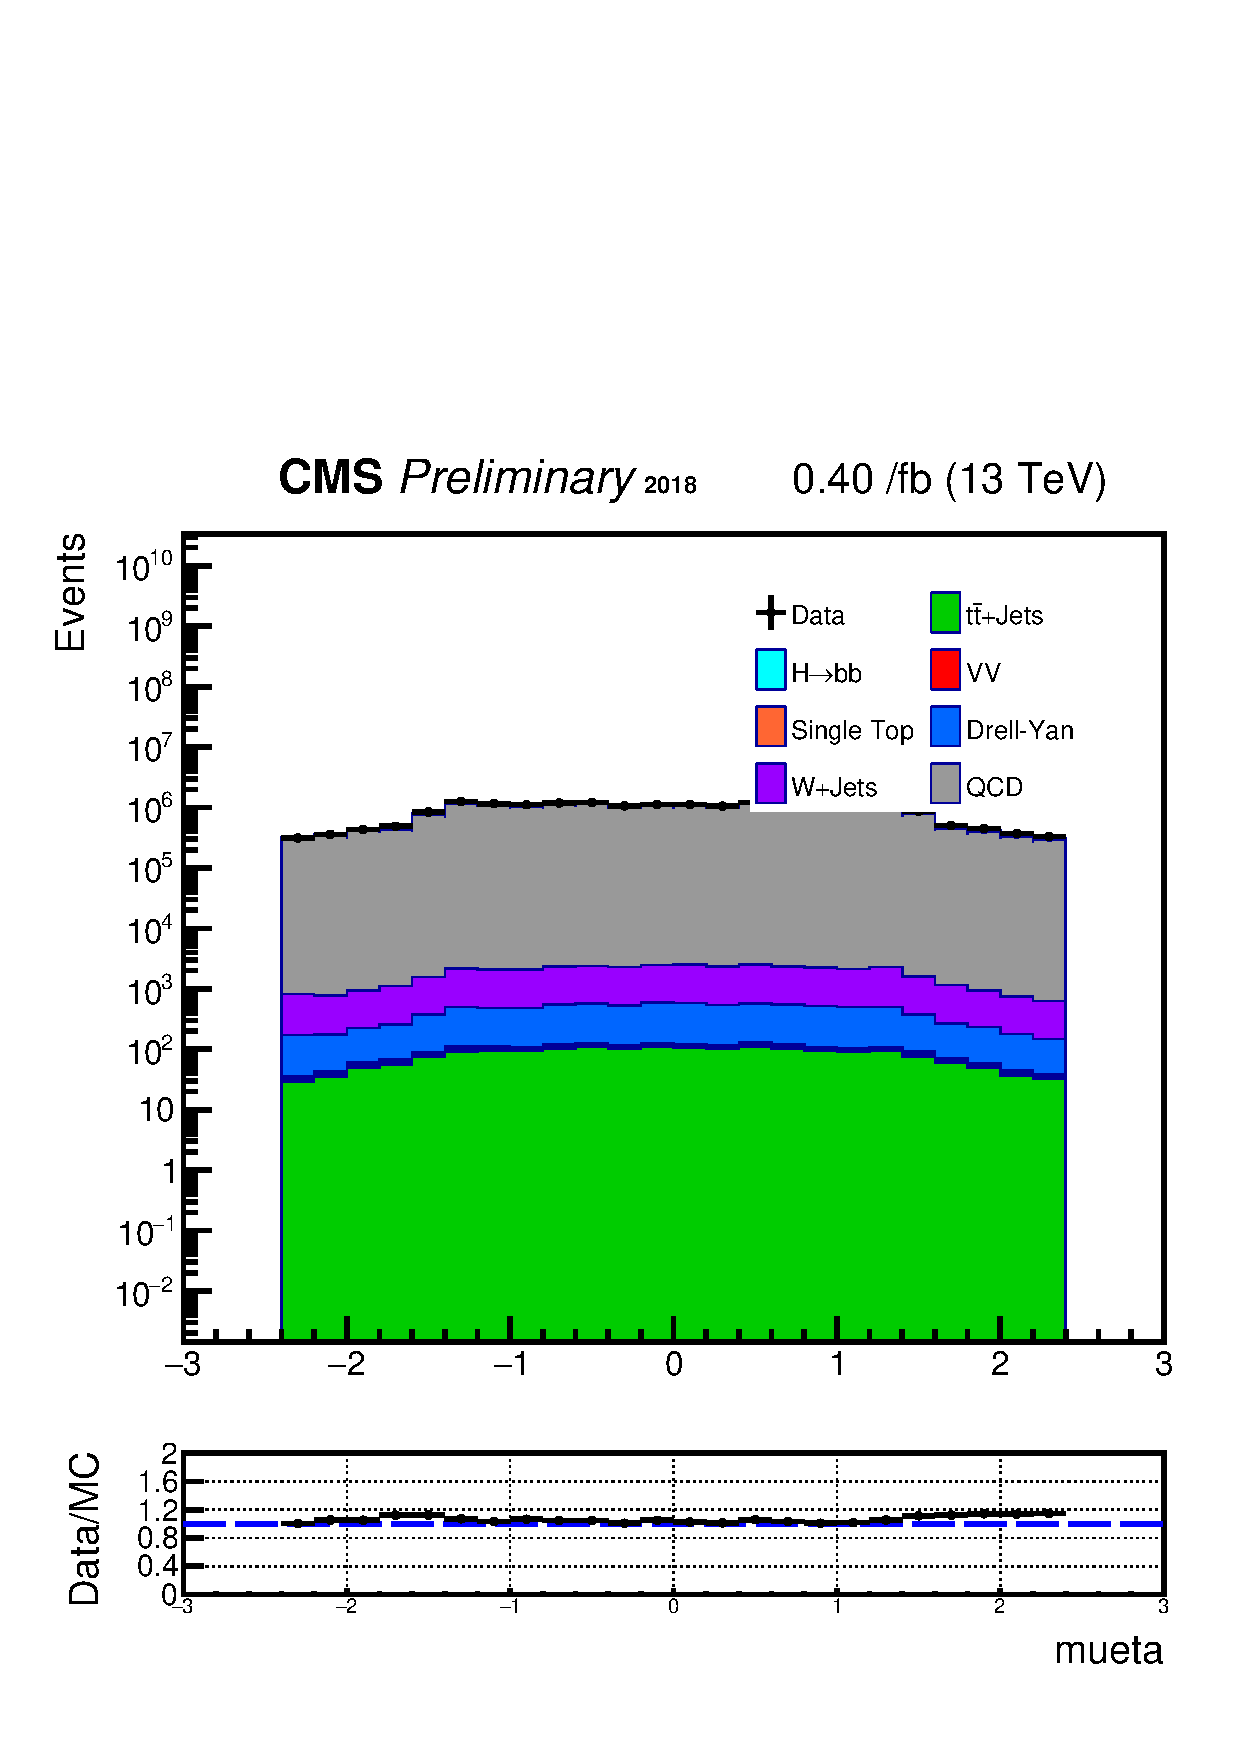
\includegraphics[width=0.47\linewidth]{figs/Data_AnalysisNoteplot_MS-15_ctauS-10_mueta.pdf}
\end{figure}

The motivations for isolation requirements on muons are further discussed in Section~\ref{sec:selections}.


\section{Jets}\label{sec:jets}

The analysis sources SlimmedJets collection from MINIAOD dataset to produce {\tt selectedJets}.
CMS reconstructs jets from calorimeter energy deposits using the
anti-$k_T$ clustering algorithm with a distance parameter of $R=0.4$~\cite{Cacciari:2008gp}.
Then, the calojets are inputed into the Particle-Flow (PF) algorithms to produce the PFJets collection. Variables in PFJets class are then slimmed to be saved into MINIAOD files. 
%The analysis uses these SlimmedJets for the jets' b tagging scores as well.
Jet objects require
\begin{itemize}
  \item pt $\geq$ 20 GeV
  \item $|\eta|$ $\leq$ 2.4
  \item 0 $\leq$ emEnergyFraction $\leq$ 0.9
  \item 0 $\leq$ energyFractionHadronic $\leq$ 0.9
  \item No selected electron or muon within $\Delta R=0.4$
\end{itemize}
The energy fraction cuts above are taken from the recommended Run2 Tight jet ID
cuts for particle flow jets~\cite{jetid_2018}.
\begin{figure}[h!]
  \caption{Data/MC of jet objects}
  \label{fig:jets}
  \centering
  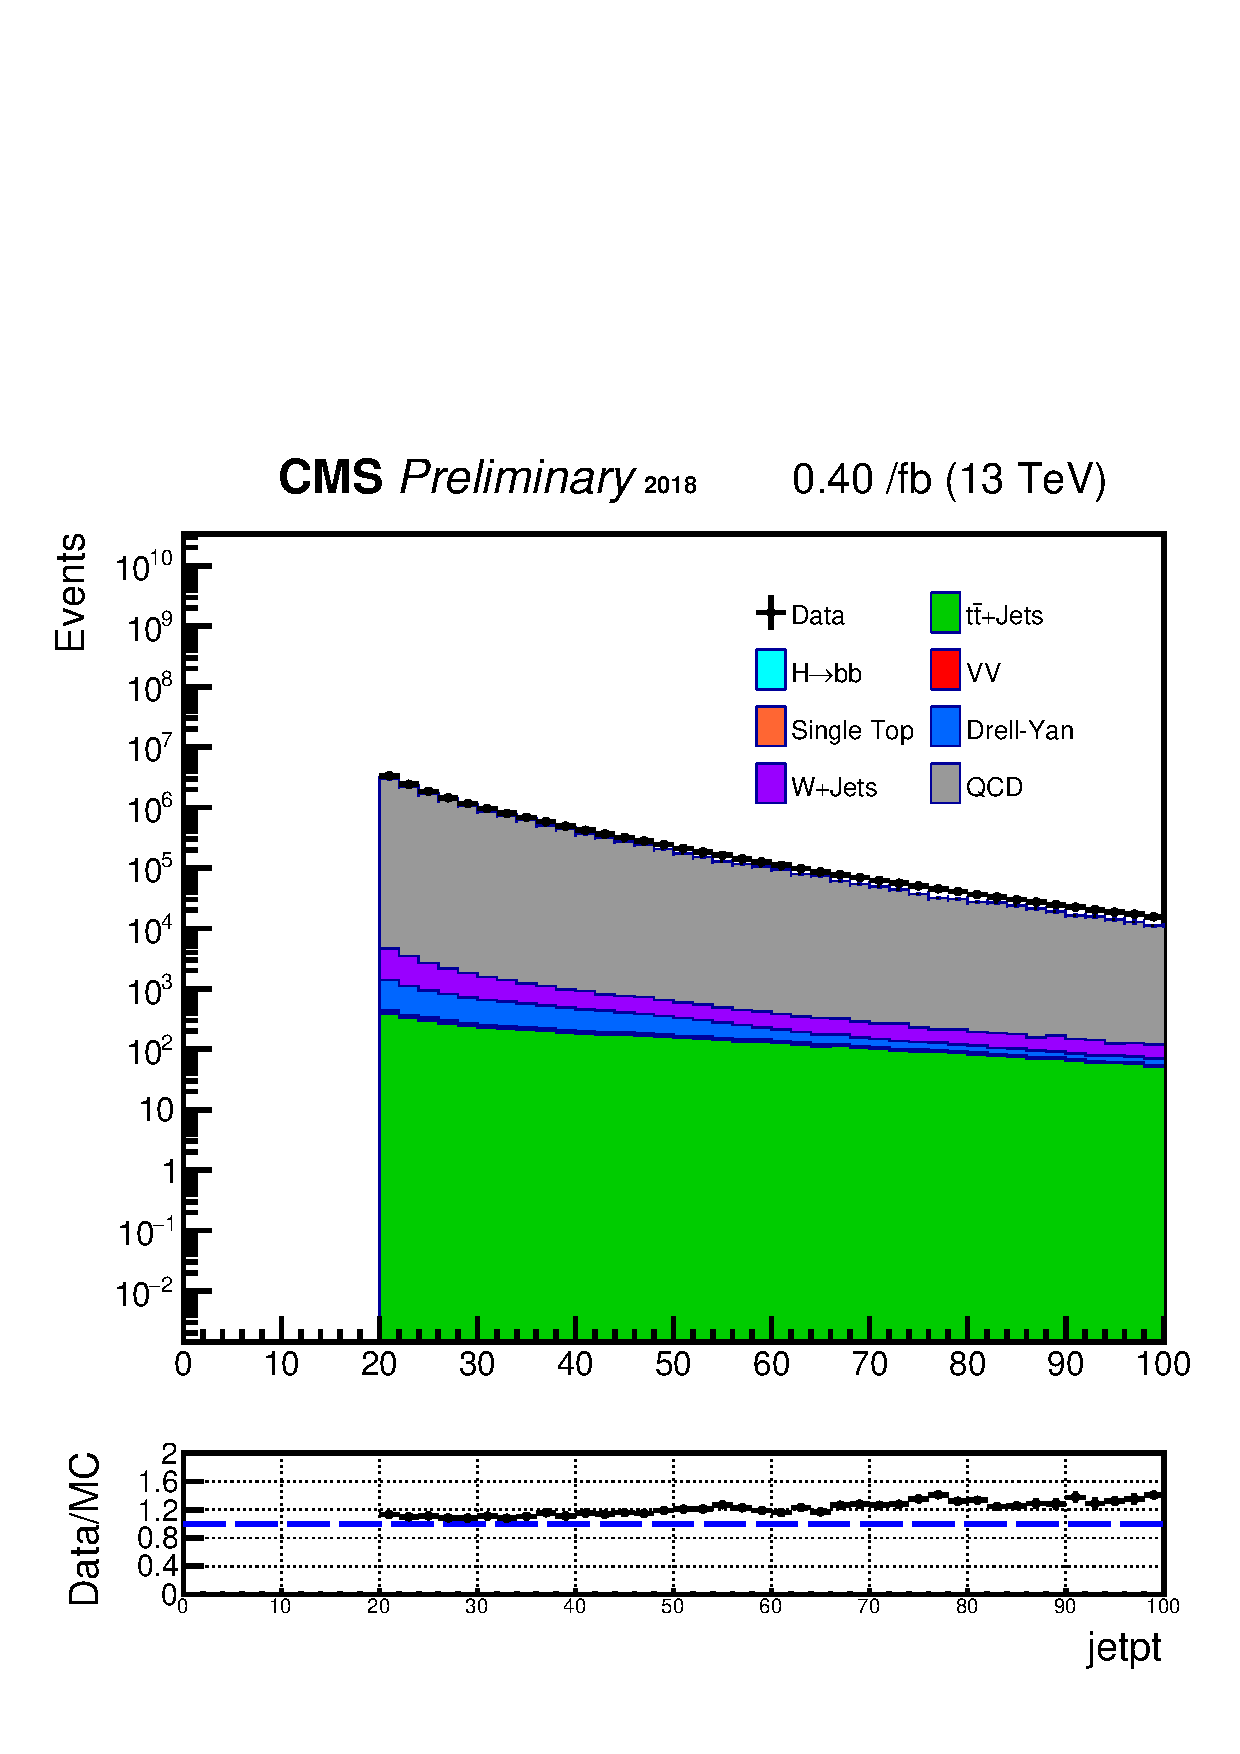
\includegraphics[width=0.47\linewidth]{figs/Data_AnalysisNoteplot_MS-15_ctauS-10_jetpt.pdf}
  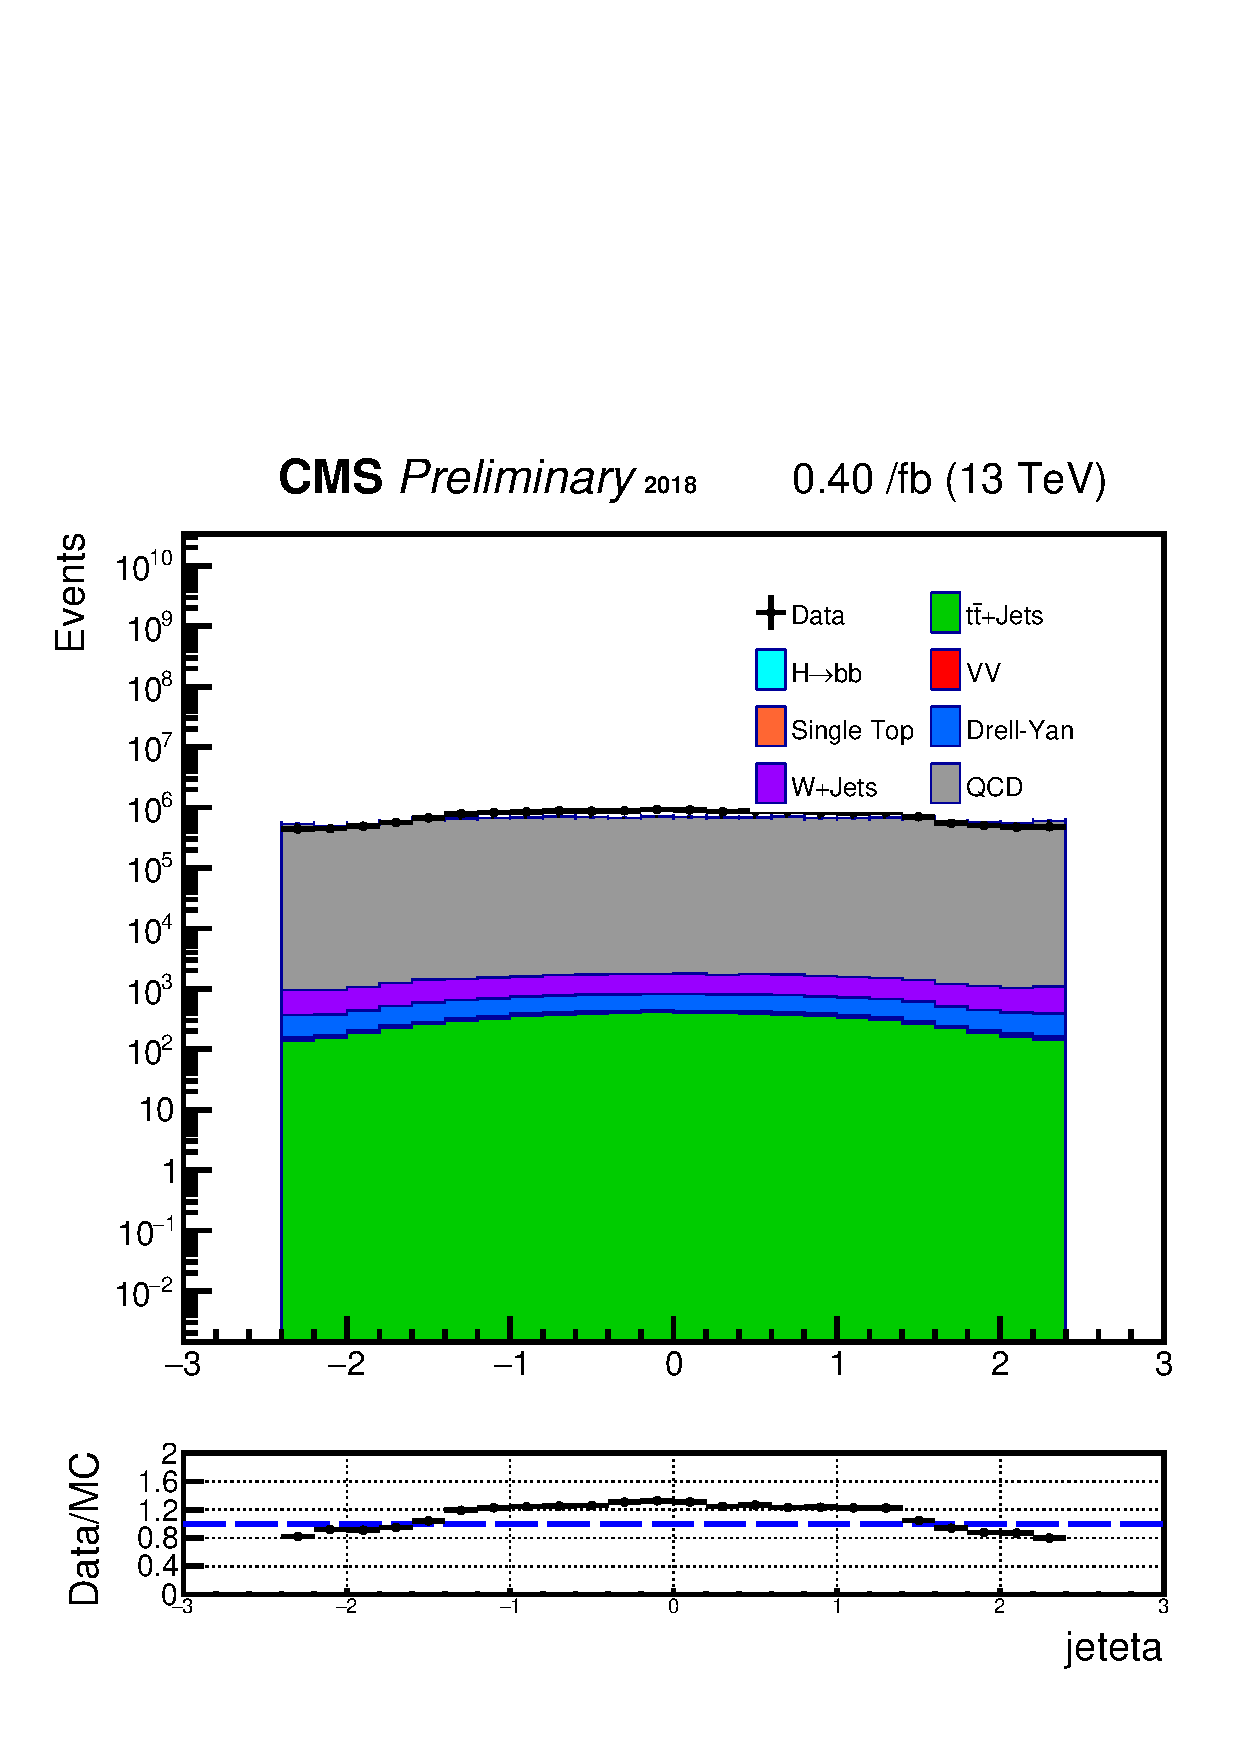
\includegraphics[width=0.47\linewidth]{figs/Data_AnalysisNoteplot_MS-15_ctauS-10_jeteta.pdf}
\end{figure}

\section{Taus}\label{sec:taus}
Although we do not use tau leptons for event selection or background estimation, we still plotted basic variables of tau leptons for review. 
The analysis sources PAT::slimmedTaus from MINIAOD for MC and RECO::slimmedTaus for Data to produce {\tt selectedTaus}.
$\tau$'s hadronic decay can be reconstructed with PFJets' charged hadrons in HCAL and 2 $\gamma$s from $\pi^{0}$ decays in ECAL.  
Tau objects require
\begin{itemize}
  \item pt $\geq$ 20 GeV
  \item $|\eta|$ $\leq$ 2.4
\end{itemize}

\begin{figure}[h!]
  \caption{Data/MC of tau objects}
  \label{fig:taus}
  \centering
  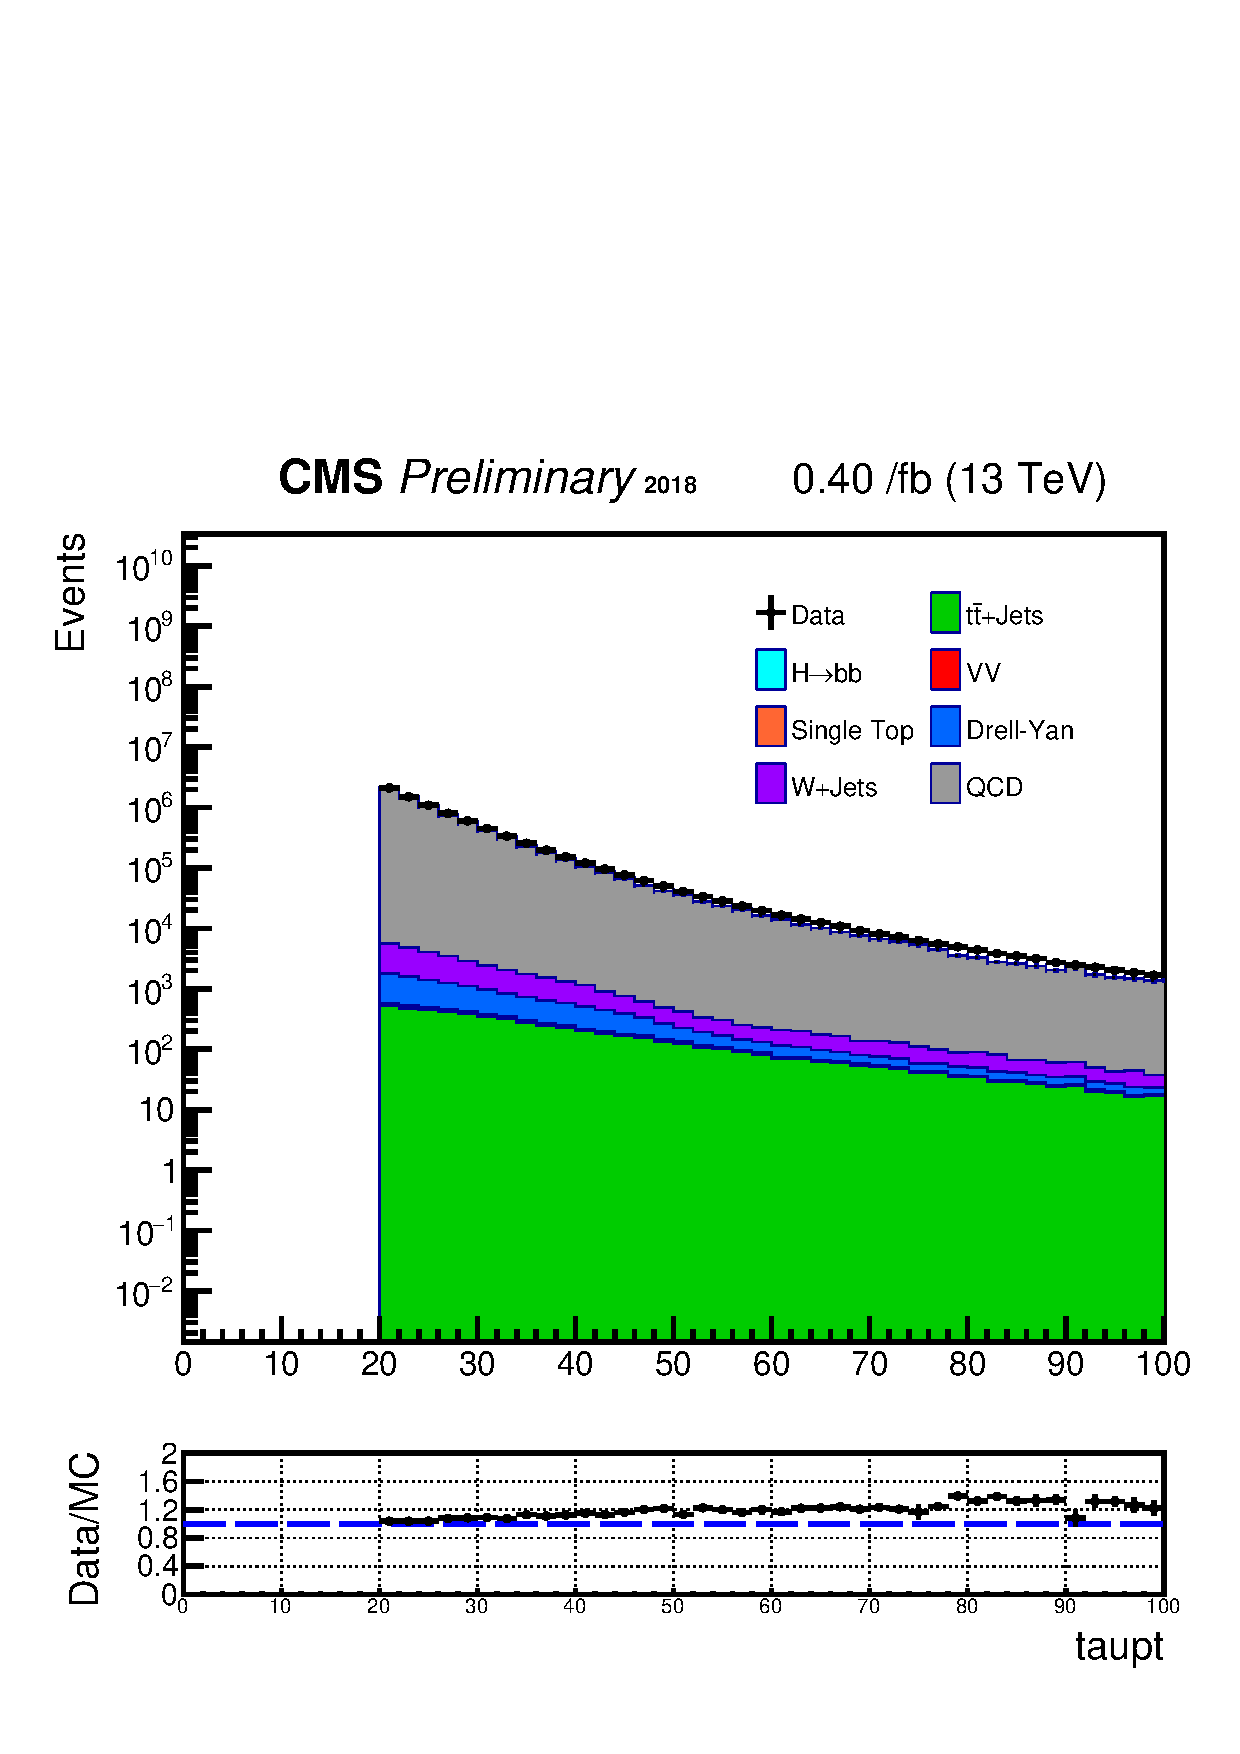
\includegraphics[width=0.47\linewidth]{figs/Data_AnalysisNoteplot_MS-15_ctauS-10_taupt.pdf}
  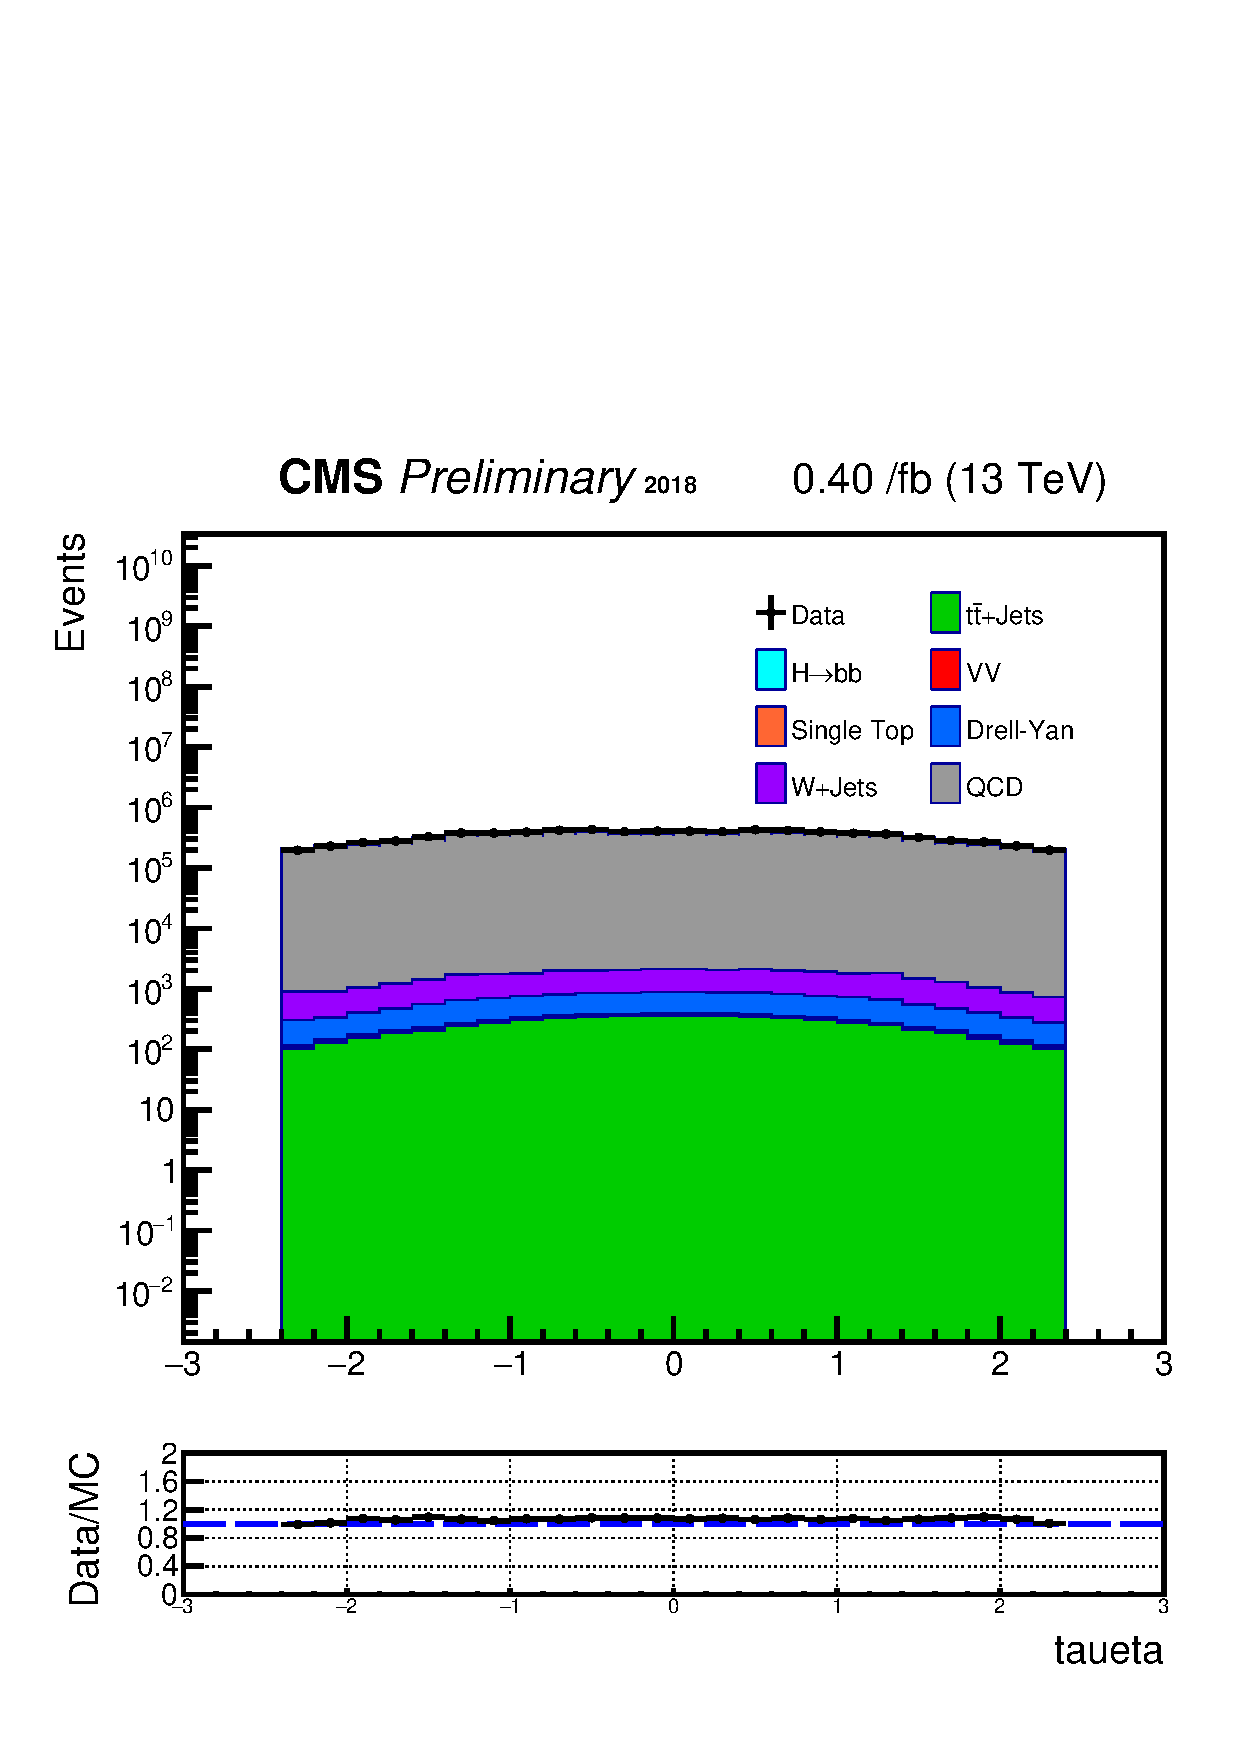
\includegraphics[width=0.47\linewidth]{figs/Data_AnalysisNoteplot_MS-15_ctauS-10_taueta.pdf}
\end{figure}





\section{Region of Interest}\label{sec:ROIs}
Tracks contain many important qualities such as the impact parameter significance and the 4 vector.
LLP scalar particles decay in the tracker, so these track qualities should be good discriminant against the background.
However, we can not save all tracks in the event with all track information, as much as we have to filter out uninteresting events with trigger system in CMS.
In our signal process, a geometrical concept can play a vital role to sort out only relevant tracks for our analysis purpose.
LLP scalar has no electric or color charge as described in section \ref{sec:theory}.
LLP scalar leaves no tracks in the tracker, decay into 2 charged tau leptons, which subsequently decay into at least 1 charged track ($\mu$, electron, at least 1 charged hadron). 
Like in the pair production, 2 charged tracks often travel opposite in their direction.
Thus, a geometric convergence of 2 charged tracks should point to the decay vertex of the neutral LLP.
The tracker algorithm that we use to construct this "Interesting Geometric Region" provides us a converged vertex, and the area around this vertex is referred as "Region of Interest" (ROI).
The complete reconstruction procedure of Regions of Interest is detailed in the following subsections.

An ROI requires
\begin{itemize}
  \item Good quality track selection
  \item Vertex Fitted from pair-wise tracks by V0Fitter in CMSSW
  \item Cluster the fitted vertices to form a Region of Intrest (ROI)
  \item Look for tracks around $\Delta R=0.3$ around ROI to save its isolation information
\end{itemize}

\subsection{Tracks}\label{sec:ROI_tracks}

The analysis sources packedPFCandidates and lostTracks from MINIAOD.
Track parameters and convariance values will be propagated along the ROI production process and no value should be non-physical
\begin{itemize}
  \item !isinf(tracks.parameter)  and !isnan(tracks.parameter) 
  \item !isinf(tracks.covariance) and !isnan(tracks.covariance) 
  \item Number of valid hits $>$ 3
  \item pt $\geq$ 0.35
  \item Track $IPSig_{XY}\geq$2.
  \item Track $IPSig_{Z}\geq$-1.
  \item Track normalized $\chi^{2}\geq$10.
\end{itemize}


\subsection{Vertex Fitter}\label{sec:ROI_V0Fitter}

The analysis sources offlineBeamspot from MINIAOD for beamspot reference.
Vertex fitter is KalmanVertexFitter with vertex cuts as below.
\begin{itemize}
  \item Vertex $\chi^{2}\geq$6.63 
  \item Transverse Decay distance significance$\geq$15.
  \item V0mass $\geq$13000GeV
  \item cos($\theta_{XY}$) between x and p of V0 candidate $\geq$ 0
  \item cos($\theta_{XYZ}$) between x and p of V0 candidate $\geq$ -2
\end{itemize}
%New PVtight and opposite traveling track req

\subsection{ROI formation}\label{sec:ROI_ROIformation}
Fitted vertices are clustered to form a Region of Interest (ROI).
The clustering steps can be further detailed as below.
\begin{itemize}
  \item A fitted vertex is merged with another vertex if they are within 1cm. 
  \item A new ROI is formed where the position vector of ROI is averaged.
  \item Clustering is repeated until there is no other vertex within 1cm limit.
\end{itemize}

Although vertex clustering can be done with the step above, we can be creative and acquire more information.
Isolation, containing information about the ROI's environment, could also be a useful information.
We can obtain information about isolation by defining an isolation shell.
The shell's construction step is described as below.
\begin{itemize}
  \item A cone of DeltaR < 0.3 around the center of the ROI is defined, where DeltaR is calculated with respect to the PV. 
  \item	A plane that is perpendicular to the axis of the cone and that contains the center of the ROI is isolation plane. It becomes a circle. 
  \item You make the circle into 3D sphere.
  \item Any tracks that pass through that sphere but not through the ROI are the annulus tracks.
\end{itemize}
With these crucial tracks' information, we are ready to discriminate signals from the background.


\begin{figure}[h!]
  \caption{Data/MC of ROI distribution}
  \label{fig:ROIs}
  \centering
  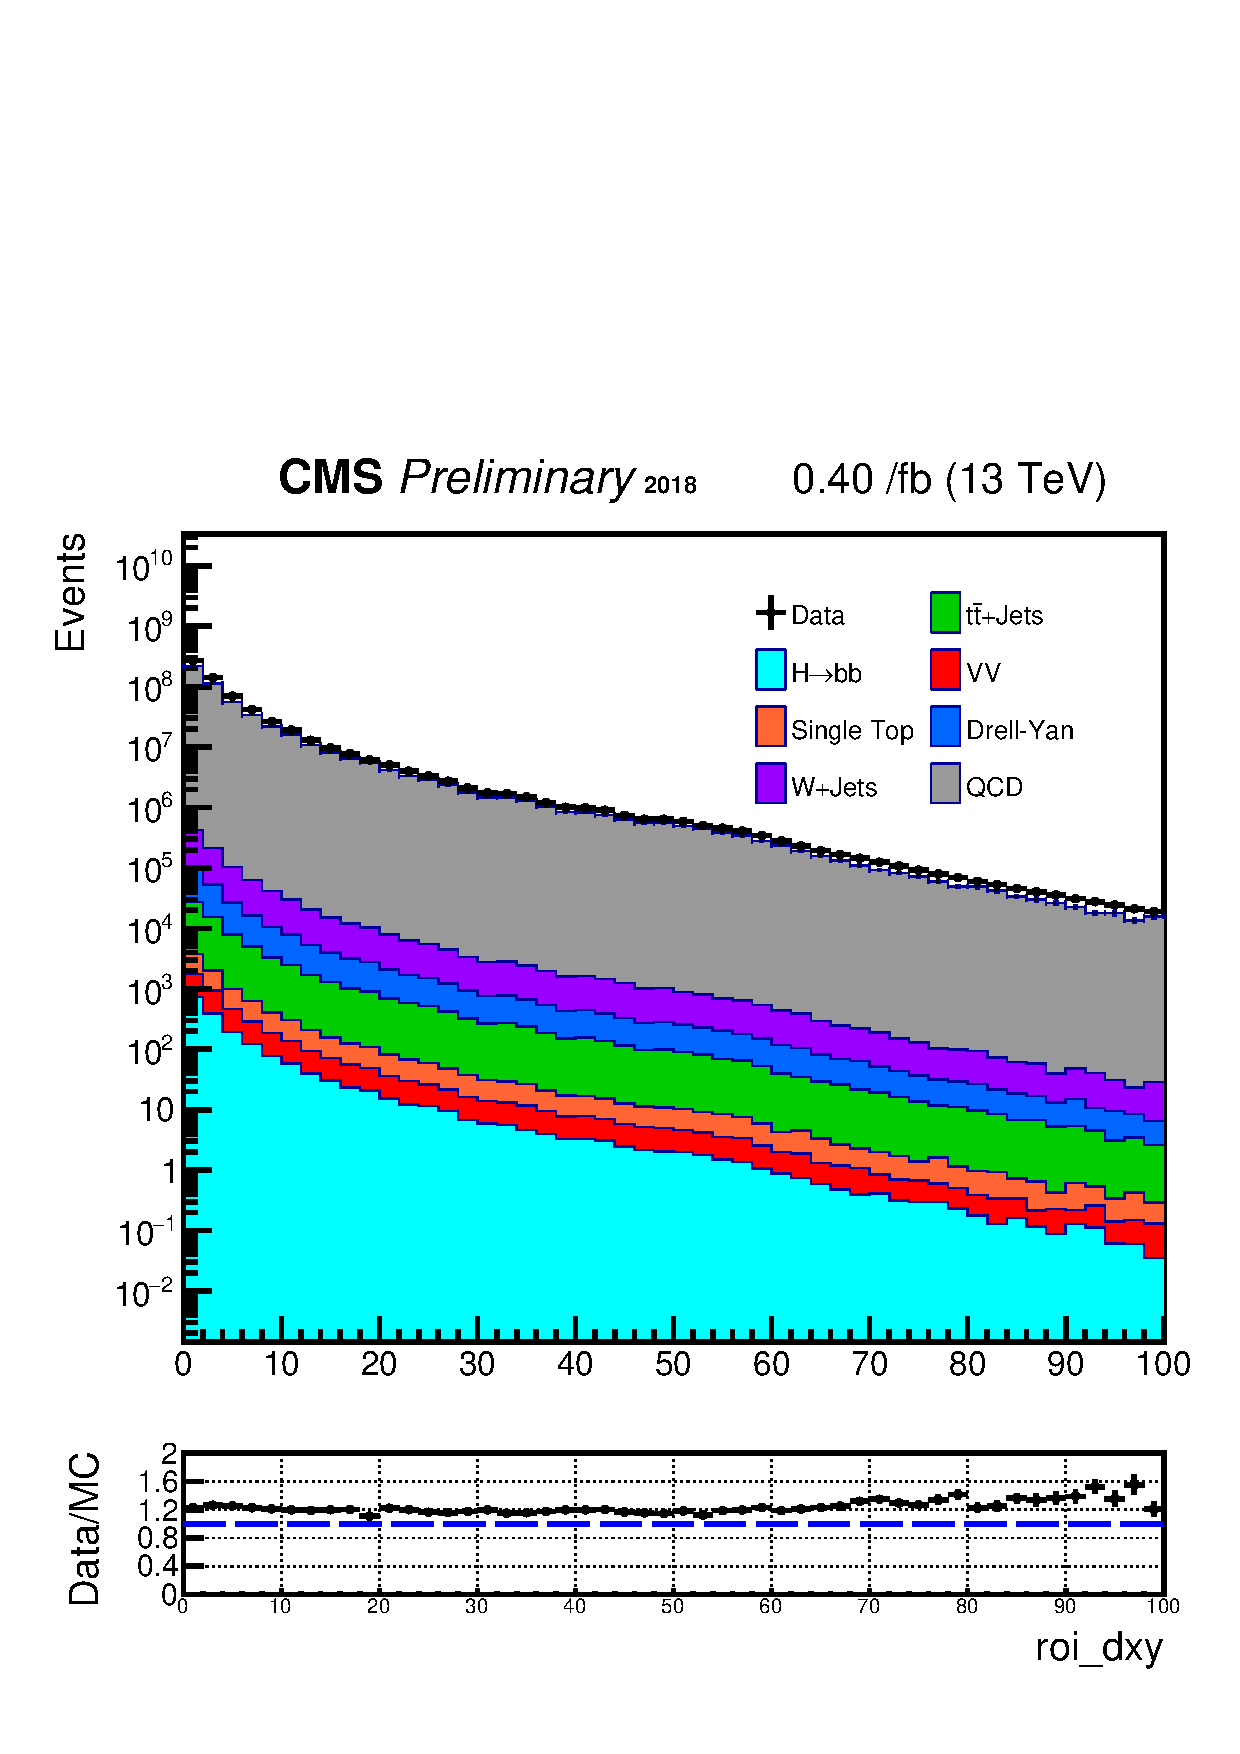
\includegraphics[width=0.47\linewidth]{figs/Data_AnalysisNoteplot_MS-15_ctauS-10_roi_dxy.pdf}
  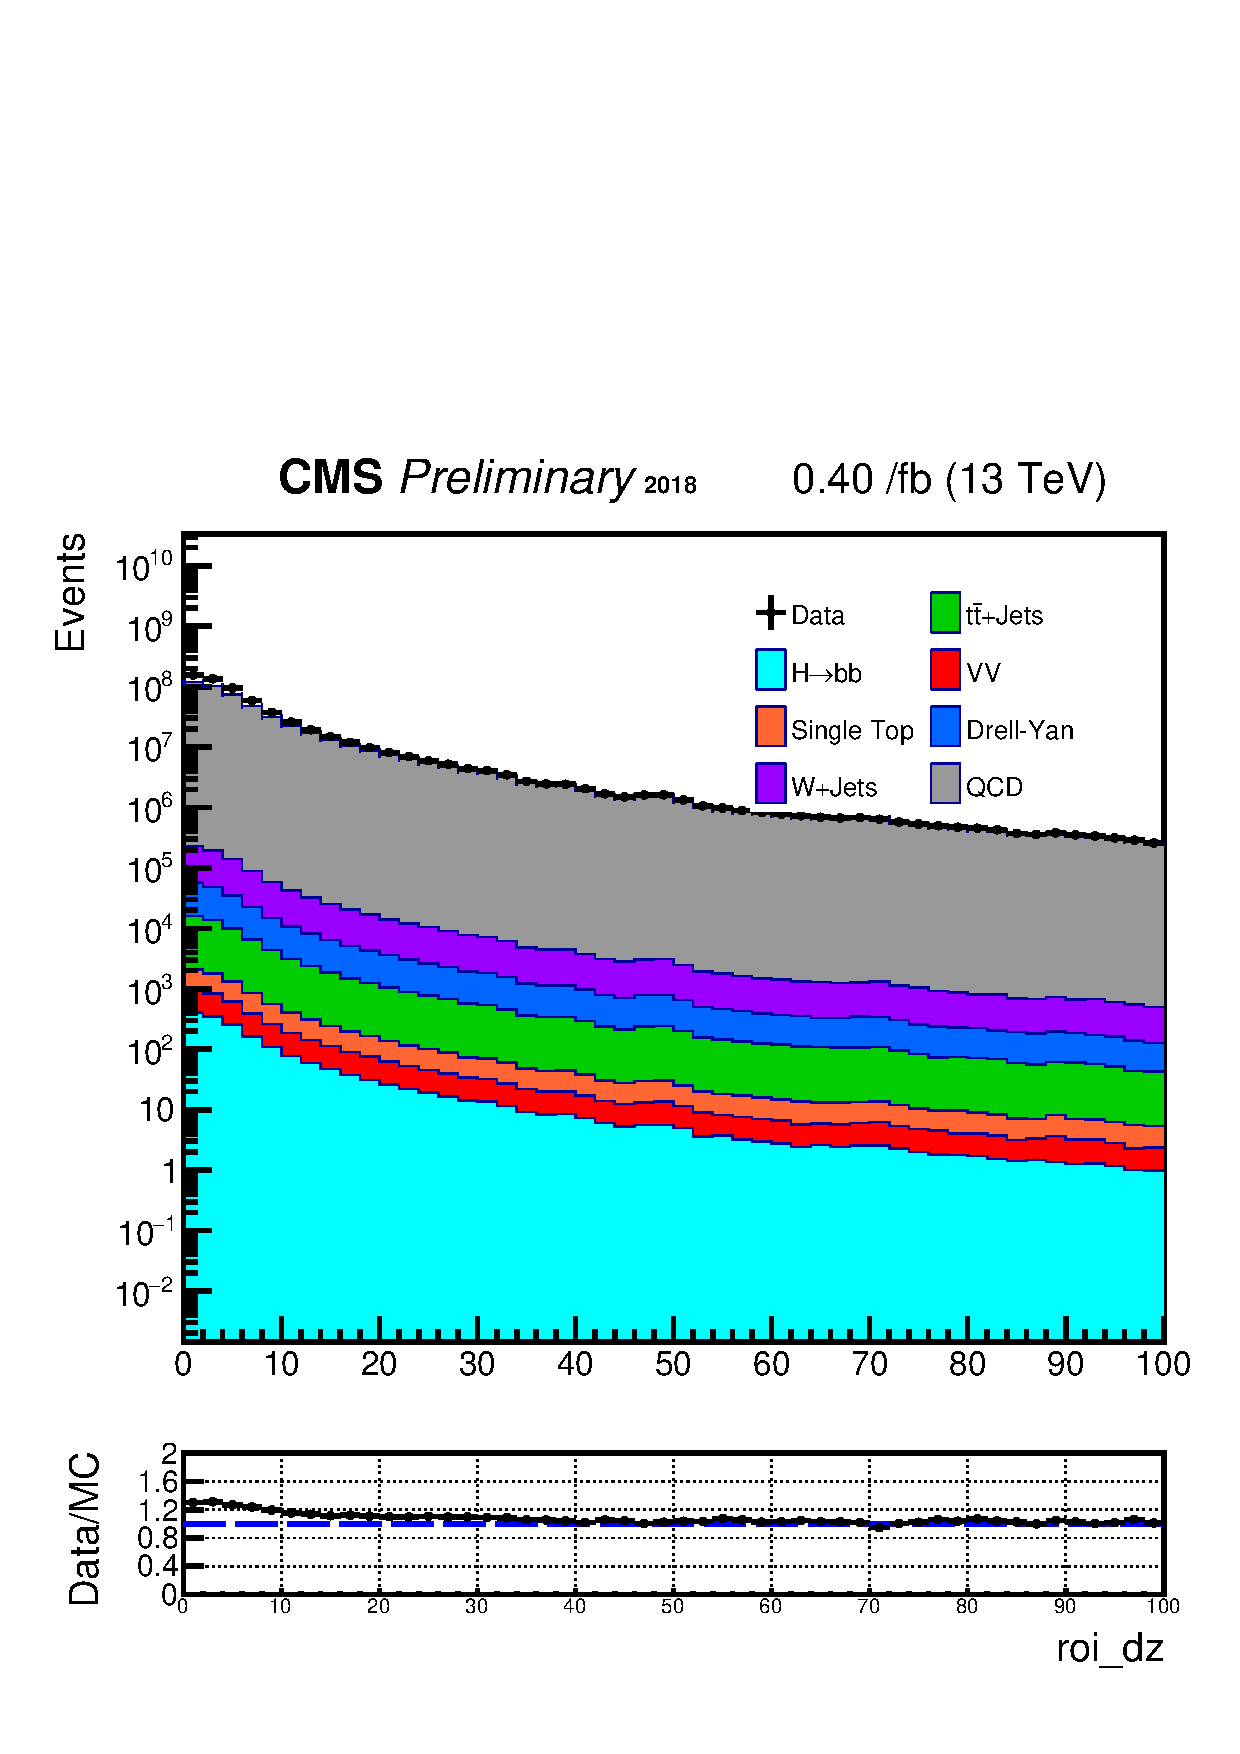
\includegraphics[width=0.47\linewidth]{figs/Data_AnalysisNoteplot_MS-15_ctauS-10_roi_dz.pdf}
\end{figure}

\begin{figure}[h!]
  \caption{2Data/MC of ROI distribution}
  \label{fig:2ROIs}
  \centering
  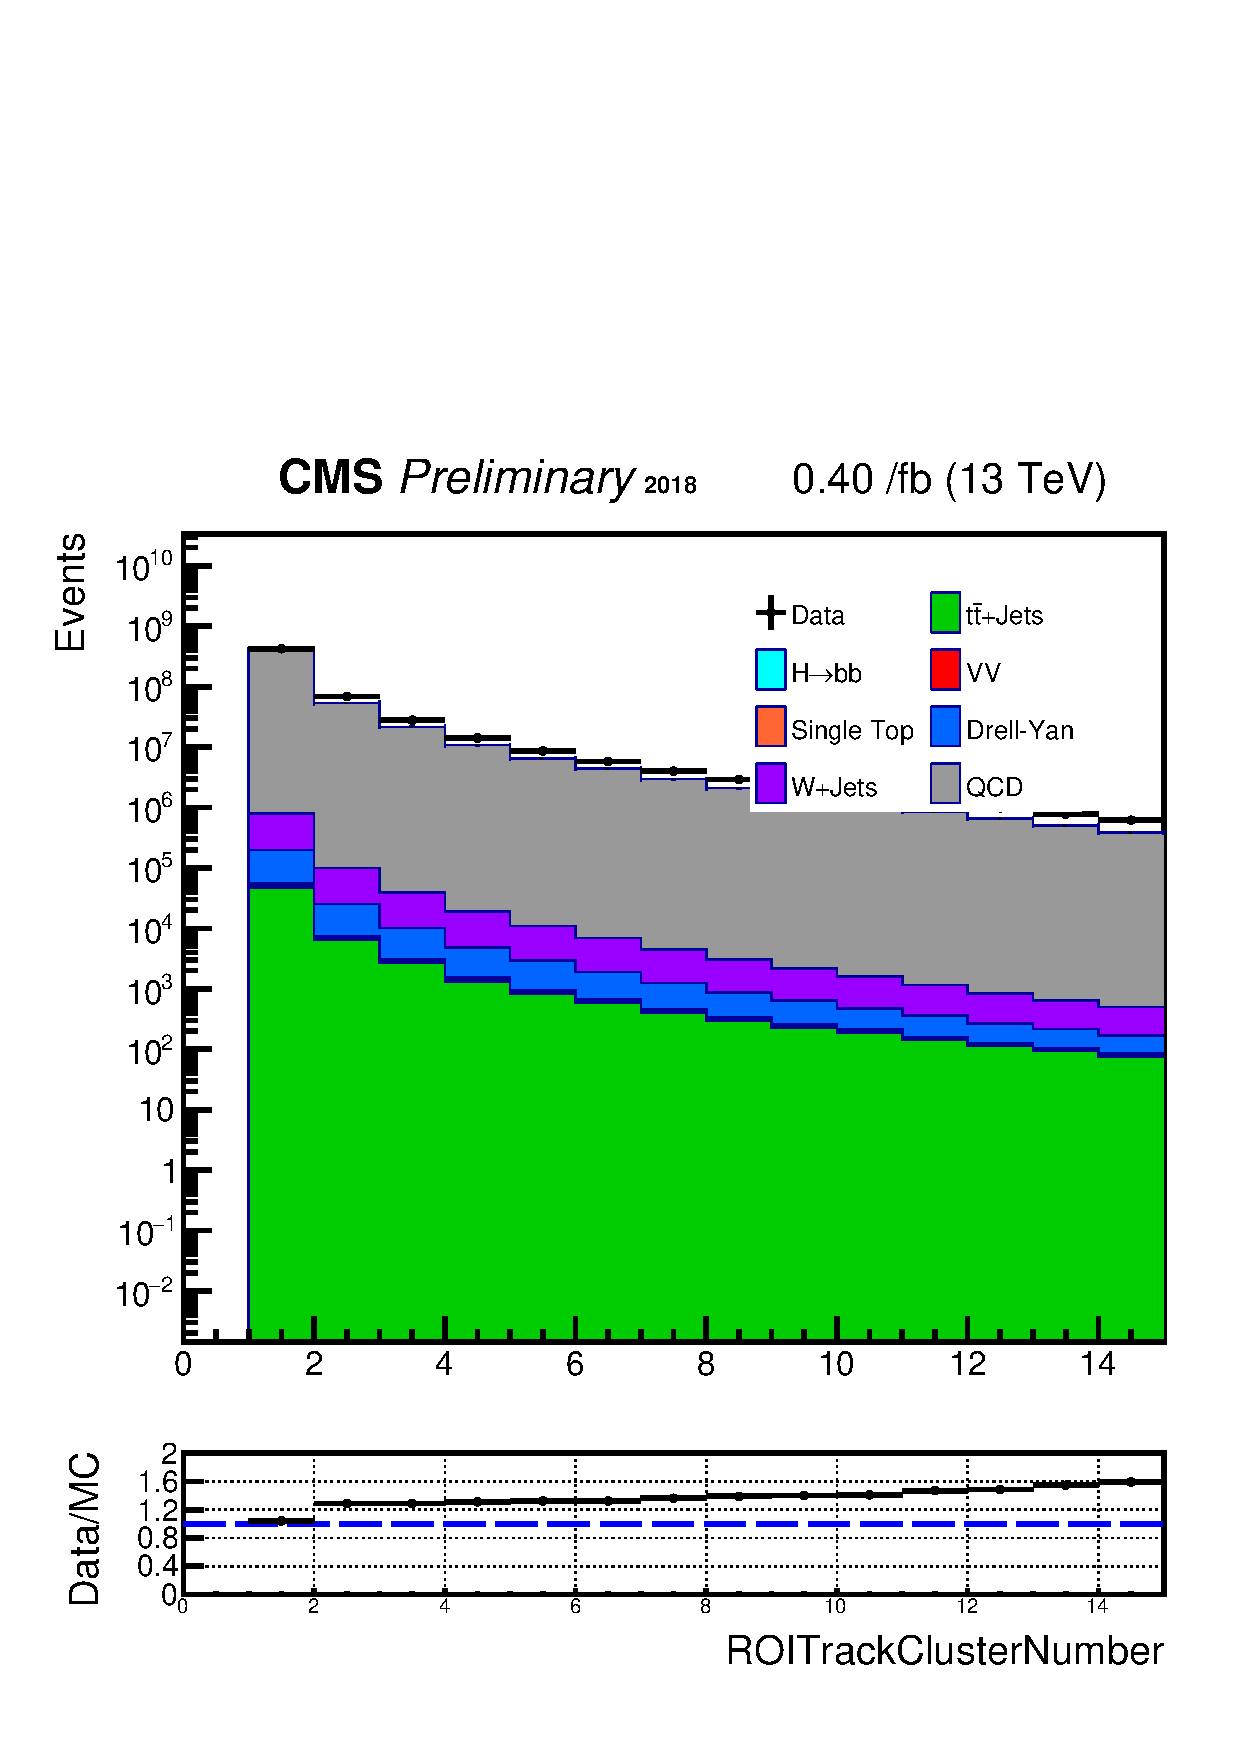
\includegraphics[width=0.47\linewidth]{figs/Data_AnalysisNoteplot_MS-15_ctauS-10_ROITrackClusterNumber.pdf}
  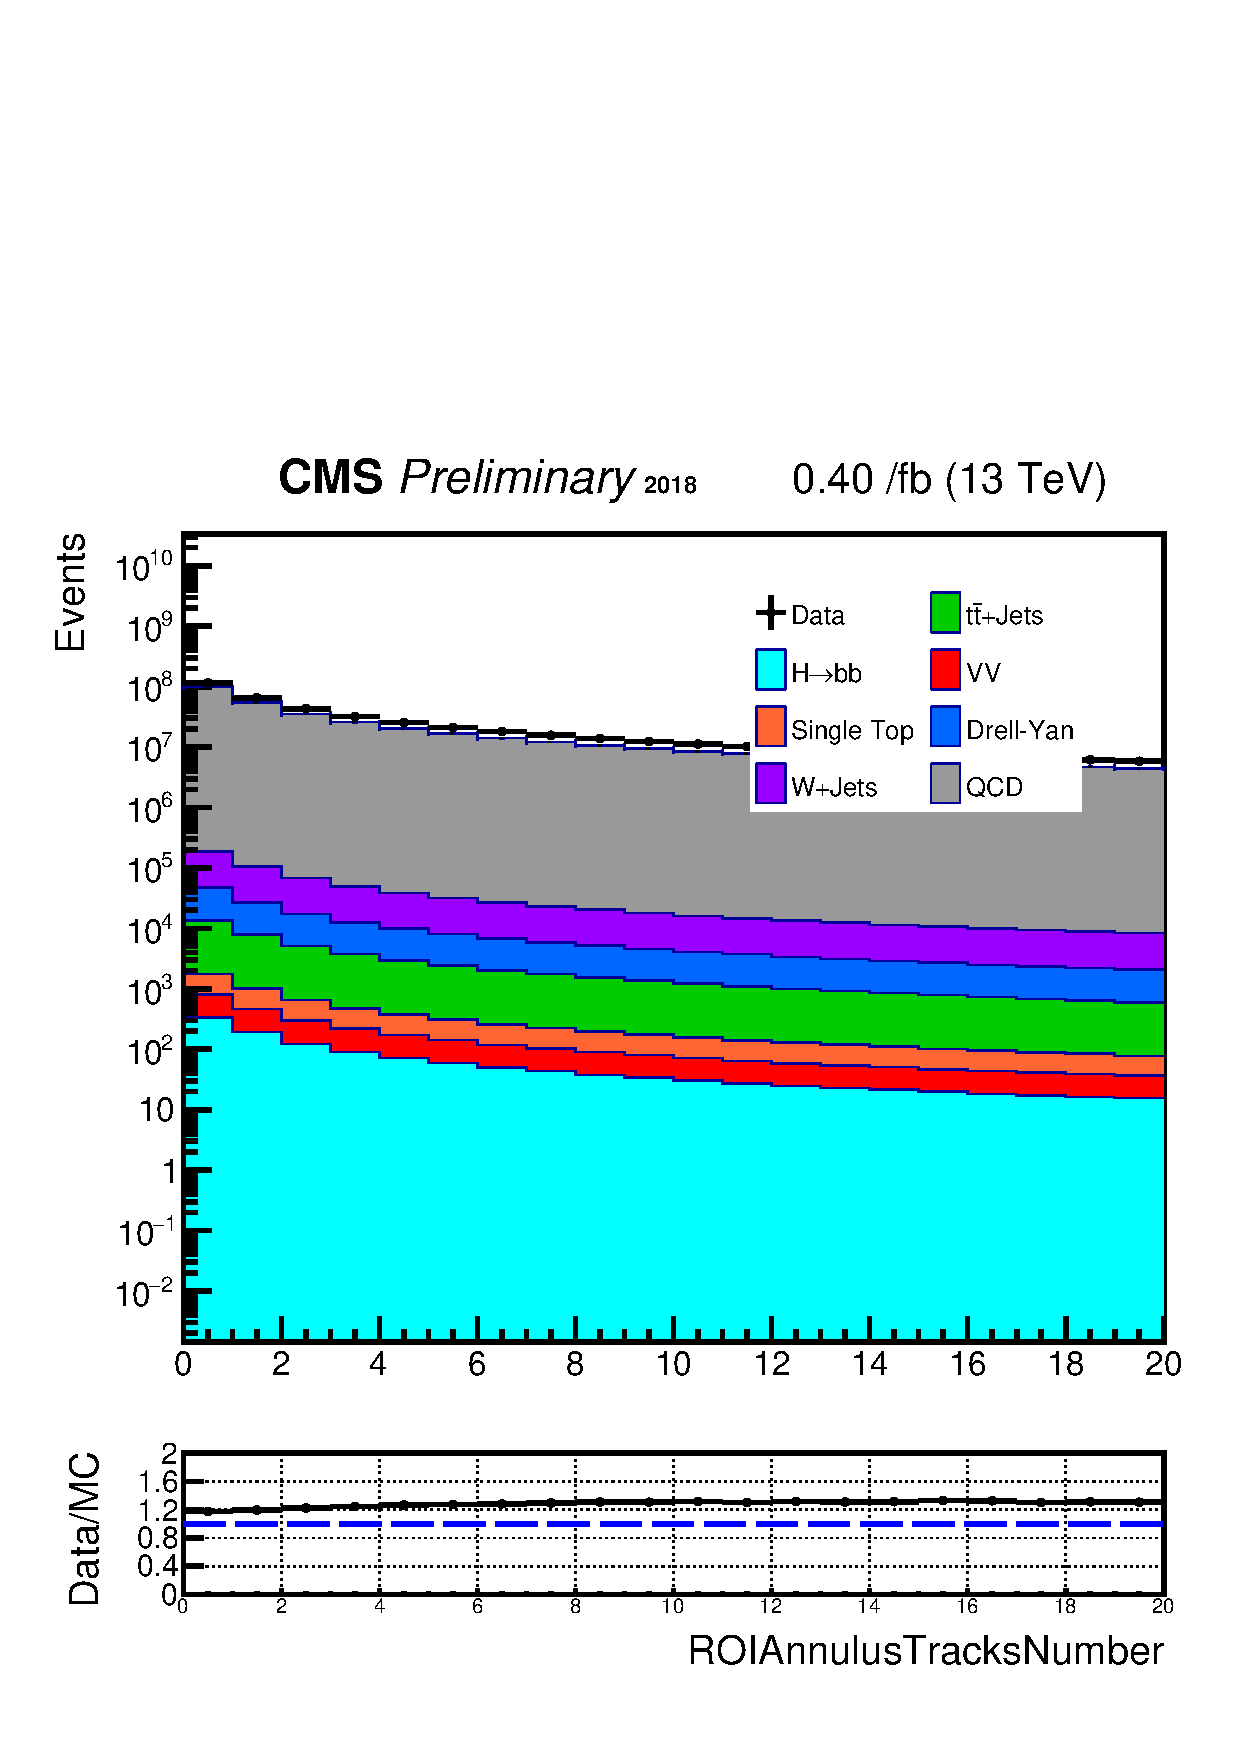
\includegraphics[width=0.47\linewidth]{figs/Data_AnalysisNoteplot_MS-15_ctauS-10_ROIAnnulusTracksNumber.pdf}
\end{figure}
